\documentclass{UoNMCHA}
\usepackage[authoryear]{natbib}
\usepackage{array,booktabs} % For nice tables
\usepackage{amsmath,amsfonts,amssymb} % For nice maths
\usepackage{color}
\usepackage{enumerate}
\usepackage{listings}
\usepackage{subfig}
\usepackage{hyperref}
\usepackage[parfill]{parskip}   % For replacing paragraph indenting with a newline instead
\usepackage{pdfpages}
\usepackage[australian]{babel} % This line sets the language to Australian English



% Number equations per section
\numberwithin{equation}{section}

\hypersetup{
%    bookmarks=true,         % show bookmarks bar?
%    unicode=false,          % non-Latin characters in AcrobatÕs bookmarks
%    pdftoolbar=true,        % show AcrobatÕs toolbar?
%    pdfmenubar=true,        % show AcrobatÕs menu?
%    pdffitwindow=false,     % window fit to page when opened
%    pdfstartview={FitH},    % fits the width of the page to the window
%    pdftitle={My title},    % title
%    pdfauthor={Author},     % author
%    pdfsubject={Subject},   % subject of the document
%    pdfcreator={Creator},   % creator of the document
%    pdfproducer={Producer}, % producer of the document
%    pdfkeywords={keyword1} {key2} {key3}, % list of keywords
%    pdfnewwindow=true,      % links in new window
    colorlinks=true,       % false: boxed links; true: colored links
    linkcolor=blue,          % color of internal links
    citecolor=blue,        % color of links to bibliography
%    filecolor=magenta,      % color of file links
    urlcolor=blue           % color of external links
}

\definecolor{MATLABKeyword}{rgb}{0,0,1}
\definecolor{MATLABComment}{rgb}{0.1328125,0.54296875,0.1328125}
\definecolor{MATLABString}{rgb}{0.625,0.125,0.9375}

\lstset{language=Matlab,
    basicstyle=\small\ttfamily,
    keywordstyle=\color{MATLABKeyword},
    %identifierstyle=,
    commentstyle=\color{MATLABComment},
    stringstyle=\color{MATLABString},
    numberstyle=\tiny,
    %numbers=left,
    basewidth=0.5em}



\firstpage{1}    % Set page number for first page
\UoNMCHAreportNo{MECH4841 Part A [B]} %Report number
\UoNMCHAyear{2013}   % Year
\shorttitle{FYP Report - Short Title} %For odd pages
%%%%%%%%%%%%%%%%%%%%%%%%%%%%%%%%%%%%%%%%%%%%%%%%%%%%
% Include the PDF title page


\begin{document}
\title{Autonomous Object Evasion, and Interception Using the Quanser QDrone\\ \ \\
{\small Final Year Project Report - ENGG4801A \\May 2024}}
\author[UoNMCHA]{Evan Byrne}
\address[UoNMCHA]{
Student of Mechatronics Engineering,\\
The University of Newcastle, Callaghan, NSW 2308, AUSTRALIA \\
Student Number: 3349681 \\
E-mail: \href{mailto:Evan.Byrne@uon.edu.au}{\textsf{Evan.Byrne@uon.edu.au}}}
%%%%%%%%%%%%%%%%%%%%%%%%%%%%%%%%%%%
\maketitle
\onecolumn

\vspace{-5mm}
\section*{Abstract}
\vspace{5mm}
This report focuses on a project in which the Quanser QDrone \cite{website:Quanser} is required to detect an object, specifically a ball in this scenario, and autonomously recognize and manoeuvre to either avoid or intercept it. This project explores various control systems and advanced object detection capabilities of current unmanned aerial vehicles (UAVs), aiming to enhance trajectory estimation for practical applications such as automated package retrieval and delivery. It also investigates the potential application of artificial intelligence and reinforcement learning to streamline these processes.

The current methodology for addressing this challenge involves the use of a Vicon System \cite{website:Vicon}. However, the project's ultimate goal is to achieve complete autonomy by relying solely on onboard sensors, cameras, and computational resources. Currently, MATLAB simulations show that nonlinear model predictive control (NMPC) \cite{website:NLMPC} is able to effectively capture the states of the QDrone; however, the processing time required with this approach has not yet been tested alongside ROS and Gazebo \cite{website:ROSandGazebo}.

\textcolor{red}{Update as you research more}

\newpage
\tableofcontents
\newpage
%%%%%%%%%%%%%%%%%%%%%%%%%%%%%%%
\section{Introduction}
To organise your introduction section you can use the following structure:
\begin{itemize}
    \item \textbf{Position}: Show there is a problem and that it is important to solve it.
    \item \textbf{Problem}: Describe the specifics of the problem you are trying to address
    \item \textbf{Proposal}: Discuss how you are going to address this problem. Use the literature to back-up your approach to the problem, or to highlight that what you are doing has not been done before
\end{itemize}
Here you need to sell why what you are doing is important, and what benefits will it bring if you are successful and solve the problem? 



%%%%%%%%%%%%%%%%%%%%%%%%%%%%%%%
\section{Literature Review}
\subsection{System Dynamics}
\subsubsection{Quadrotor Dynamics}
\subsubsection{Object Dynamics}
\subsection{Control Strategy}
\subsubsection{PD Control}
\subsubsection{PID Control}
\subsubsection{LQR Control}
\subsubsection{MPC}
\subsubsection{NMPC}
\subsection{Trajectory Prediction}
\subsubsection{Kalman Filter}
\subsubsection{Extended Kalman Filter}
\subsubsection{Unscented Kalman Filter}
\subsection{Reinforcement Learning}
\subsubsection{Model Based RL}
\subsubsection{Model Free RL}
\subsubsection{PPO(Proximal Policy Optimization)}


\section{Quadrotor System Modelling}
\subsection{System Representation}
\subsubsection{Assumptions}
\subsubsection{Coordinates and Rotation Matricies}
\subsubsection{States and Inputs}
\subsection{Motor Equations}
\subsection{Translational Dynamics}
\subsection{Rotational Dynamics}
\subsection{State Space Equations of Motion}

\section{Object System Modelling}

\section{Control Strategy}
\subsection{Overview}
\subsection{PID}
\subsection{MPC}
\subsection{NMPC}








\LaTeX \ is very good for writing Mathematics. You can write mathematics in the middle of a sentence, like for example $y=m x + h$. Or you can use the \verb|equation| environment as indicated in \eqref{eq:EquationLine} below.
\begin{equation}\label{eq:EquationLine}
    y=m x + h.
\end{equation}
You can also use equations and tell LaTeX not to number an equation:
\begin{equation*}
    z=m_z x^2 + h_z.
\end{equation*}
You can use the split command as in \eqref{eq:SS1} below (split gives you only one equation number):
\begin{equation}\label{eq:SS1}
    \begin{split}
        \dot{\mathbf{x}} &= \mathbf{A} \mathbf{x} + \mathbf{B} \mathbf{u}, \\
        \mathbf{y} &= \mathbf{C} \mathbf{x} + \mathbf{D} \mathbf{u},
    \end{split}
\end{equation}
and you also use numbers for each equation and refer to them separately like in \eqref{eq:State} and \eqref{eq:Output} below:
\begin{align}
    \dot{\mathbf{x}} &= \mathbf{A} \mathbf{x} + \mathbf{B} \mathbf{u},  \label{eq:State} \\
    \mathbf{y} &= \mathbf{C} \mathbf{x} + \mathbf{D} \mathbf{u}. \label{eq:Output} 
\end{align}
You can write a matrix like
\begin{equation*}
    \mathbf{A} =
    \begin{bmatrix}
        A_{11} & A_{12} & \dots & &A_{1n} \\
        A_{21} & A_{22} &  \dots & &\vdots \\
        \vdots & \vdots & \ddots& &  \vdots\\
        A_{m1} & A_{m2} & \dots & &A_{mn}
    \end{bmatrix}.
\end{equation*}
If you want to distinguish vectors from scalars you can use \textbf{bold} for vectors and matrices:
\begin{equation*} 
    \begin{split}
        \dot{\mathbf{x}} &= \mathbf{A} \mathbf{x} + \mathbf{B} u, \\
        y &= \mathbf{C} \mathbf{x} + \mathbf{D} u,
    \end{split}
\end{equation*}
where $u$ and $y$ are scalar variables and $\mathbf{x}$ is a vector variable.
You can also write Greek letters in bold: $\boldsymbol{\alpha}$.
%%%%%%%%%%%%%%%%%%%%%%%%%%
\subsection{Figures}
To import the figures from Matlab, follow the following procedure:
\begin{enumerate}
    \item Add labels and legends (don't forget to include units in the labels of each axis.)
    \item From the file menu tag on the figure select export set up
    \item Change the font size to 14 and click apply to figure
    \item Export the figure as eps
    \item Import it in LaTeX using the include graphics within a \verb|figure| environment.
\end{enumerate}
%
\begin{figure}[ht]
    \begin{center}
        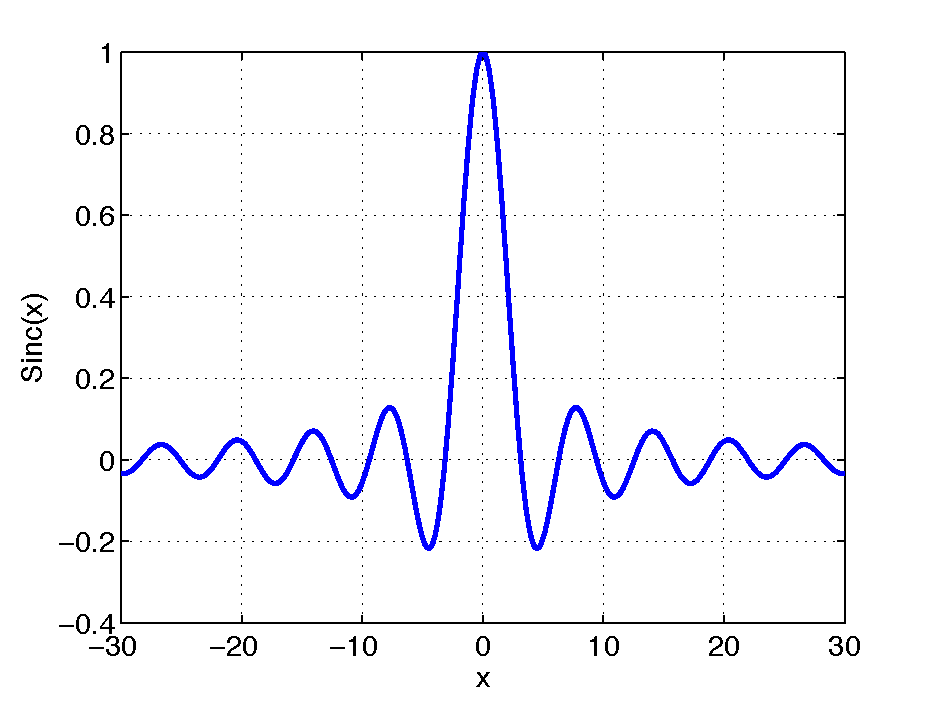
\includegraphics[width=.6\linewidth]{Figures/SincPlot}
        \caption{Here goes the caption.}
        \label{fig:Sinc}
    \end{center}
\end{figure}
Figure~\ref{fig:Sinc} shows a shows a plot of the function $\sin(x)/x$. 

If I need to make a simple diagram, I use powerpoint and select the drawing and save it as a pdf. For example, look at Figure~\ref{fig:MechaSys}.
\begin{figure}[ht]
    \begin{center}
        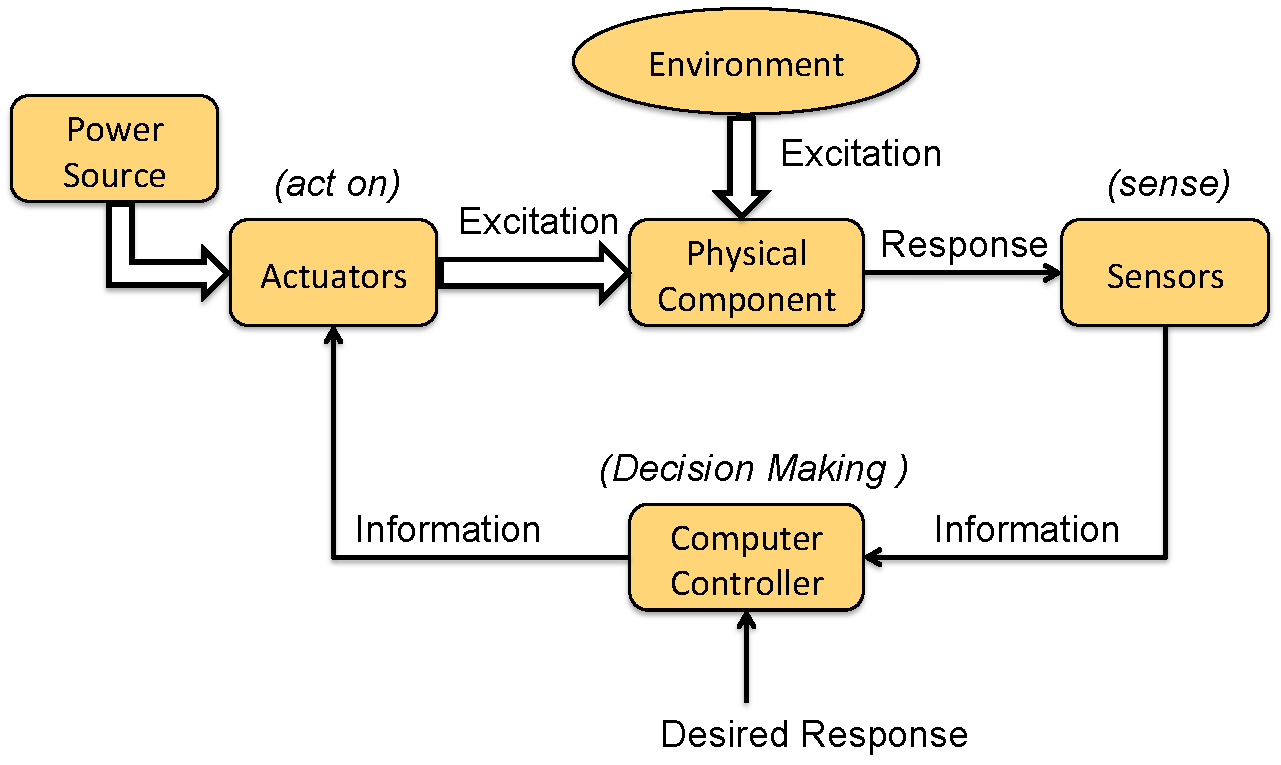
\includegraphics[width=.6\linewidth]{Figures/MechaSys}
        \caption{Here goes the caption.}
        \label{fig:MechaSys}
    \end{center}
\end{figure}
%%%%%%%
\newpage
\subsection{Lists}
To create lists use the environments \verb|itemize|, \verb|enumerate|, or \verb|description|

The following is generated using \emph{itemize}
\begin{itemize}
    \item This is item 1 
    \item This is item 2
\end{itemize}
%
The following is generated using \emph{enumerate}
\begin{enumerate}[1)]
    \item This is item 1 
    \begin{enumerate}[a)]
        \item Subitem a
        \item Subitem b
        \begin{enumerate}[i)]
            \item Subsubitem i
            \item Subsubitem ii
        \end{enumerate}
    \end{enumerate}
    \item This is item 2
\end{enumerate}
%
The following is generated using \emph{description}
\begin{description}
    \item[foo)] This is item 1 
    \item[bar)] This is item 2
\end{description}

\subsection{Code listings}

To include a syntax-highlighted code listing, you can use the \emph{listings} package. The default options are specified by the \verb|\lstset| command. There are 3 main commands, all of which can include options to override the defaults:
\begin{enumerate}
    \item \verb|\lstinline|: Command for including code fragments inline with the text, as an alternative to \verb|\verb|. For example, we might describe function prototypes such as \lstinline[language=C,breaklines=true]|int main(int argc, char *argv[])|.
    \item \verb|\begin{lstlisting}|,\ldots,\verb|\end{lstlisting}|: Environment for including a source code listing---embedded in the LaTeX source---in a box or floating environment. An example is shown in Listing~\ref{lst:sqrt}.
    \item \verb|\lstinputlisting|: Command for including a source code listing---loaded from an external file---in a box or floating environment. This method is preferred over including the code source within the LaTeX file, since the code and its documentation can always be kept in sync. An example is shown in Listing~\ref{lst:matlabserial}.
\end{enumerate}

\begin{lstlisting}[
    language=C,
    float=h,
    numbers=none,
    xleftmargin=1cm,
    frame=none,
    caption={A winning entry from the 16th International Obfuscated C Code Contest, that computes the square root of its input.\label{lst:sqrt}}
    ]
#include <stdio.h>
int l;int main(int o,char **O,
int I){char c,*D=O[1];if(o>0){
for(l=0;D[l              ];D[l
++]-=10){D   [l++]-=120;D[l]-=
110;while   (!main(0,O,l))D[l]
+=   20;   putchar((D[l]+1032)
/20   )   ;}putchar(10);}else{
c=o+     (D[I]+82)%10-(I>l/2)*
(D[I-l+I]+72)/10-9;D[I]+=I<0?0
:!(o=main(c/10,O,I-1))*((c+999
)%10-(D[I]+92)%10);}return o;}
\end{lstlisting}

\lstinputlisting[
    language=Matlab,
    float=h,
    numbers=left,
    xleftmargin=1cm,
    frame=shadowbox,
    caption={Matlab serial communication example.\label{lst:matlabserial}},
    morekeywords={try,catch}
    ]{Code/serialtest.m}

 %%%%%%%%%%%%%%%%%%%%%%%%%%%%%%%
\section{References and Citations}\label{sec:RefCite}
To generate the bibliography look at the end of this document in .tex file. To make reference to the bibliography use the commands \verb|\citet{}| and \verb|\citep{}| \citep{strunk2007elements}. You can combine more than one reference in a single citation \citep{troyka1999simon, jay1995write}.



\section{Conclusion}\label{sec:Conclusion}
This is one of the most important parts of the report. In the conclusion section, you  should 
\begin{itemize}
\item briefly summarise the results,
\item reflect on the work presented, 
\item make recommendations,
\item suggest future work or improvements.
\end{itemize}

%%%%%%%%%%%%%%%%%%%%%%%%%%%%%%%%
\bibliographystyle{harvard}
\bibliography{main} % This is the .bib file where the bibliography database is stored

\appendix
\newpage
\section{Example of a Table}\label{app:Table}
 %
\begin{table}[h!]
    \begin{center}\label{tab:MCHAProg}
        \caption{Proposed Bachelor of Engineering Mechatronics Program}\label{tab:notation}
        {\footnotesize
            \begin{tabular}{c l l l|}
                \hline\hline \textbf{1st Year} & & \\
                Semester & {Course Code} & {Course Name} \\ \hline 
                1 & GENG1000 & Computer Aided Engineering \\
                1 & GENG1803 & Introduction to Engineering Practice\\
                1 & MATH1110 & Mathematics I\\
                1 & PHYS1205 & Integrated Physics\\ \hline
                2 & ELEC1300 & Electrical Engineering I\\
                2 & \textbf{GENG1003} & \textbf{Procedural Programming}  \\
                2 & GENG1001 & Introduction to Engineering Mechanics\\
                2 & MATH1120 & Mathematics II 
                \\ \hline
                %
                \hline \textbf{2nd Year} &  \\
                Semester & {Course Code} & {Course Name} \\ \hline 
                1 & ELEC1700 & Computer Engineering I\\
                1 & ELEC2700 & Computer Engineering II\\
                1 & MECH2420 & Engineering Mechanics\\
                1 & \textbf{MCHA2440} & \textbf{Computational Engineering Modelling} \\ \hline
                2 & \textbf{MCHA2000} & \textbf{Mechatronic Systems} \\
                2 & \textbf{MECH2450} & \textbf{Engineering Computations II} \\
                2 & MECH2350 & Dynamics II\\
                2 & ELEC2320 & Electrical Circuits\\ \hline
                %
                \hline \textbf{3rd Year} &  \\
                Semester & {Course Code} & {Course Name} \\ \hline 
                1 & MECH2110 & Mechanical Engineering Design I\\
                1 & ELEC4400 & Automatic Control\\
                1 & ELEC3240 & Electronics\\
                1 & ELEC3730 & Embedded Systems \\ \hline
                2 & \textbf{MECH4400} & \textbf{Computational Mechanics}  \\
                2 & MECH2700 & Thermofluids \\
                2 & \textbf{MCHA3000} & \textbf{Mechatronic System Design I} \\
                2 & \textbf{ELEC4410} & \textbf{Control System Design and Management}   \\ \hline
                % 
                \hline \textbf{4th Year} &  \\
                Semester & {Course Code} & {Course Name} \\ \hline 
                1 & \textbf{MCHA3900} & \textbf{Mechatronic System Design II} \\
                1 & PHIL3910 & Technology and Human Values\\
                1 & GENG3830& Engineering Project Management\\
                1 & FYP A & Final Year Project part A\\ \hline
                2 & GE & General Elective\\
                2 & GE & General Elective\\
                2 & FYP B & Final Year Project part B \\ \hline
            \end{tabular}
        }
    \end{center}
\end{table}
Courses in \textbf{bold} are new to the program.

\end{document}
